% SOURCE: submissions/d2-neurocomputing/zenodo-deposit/results/merging/RG_map_evidence_REFIX20260801.json :: cells.*.per_g.{2,3,5,10,20}.partial_rho_{s0,s1,s2,mean}; facets cells.*.regime; gate line partial=0.15
% !TEX encoding = UTF-8 Unicode
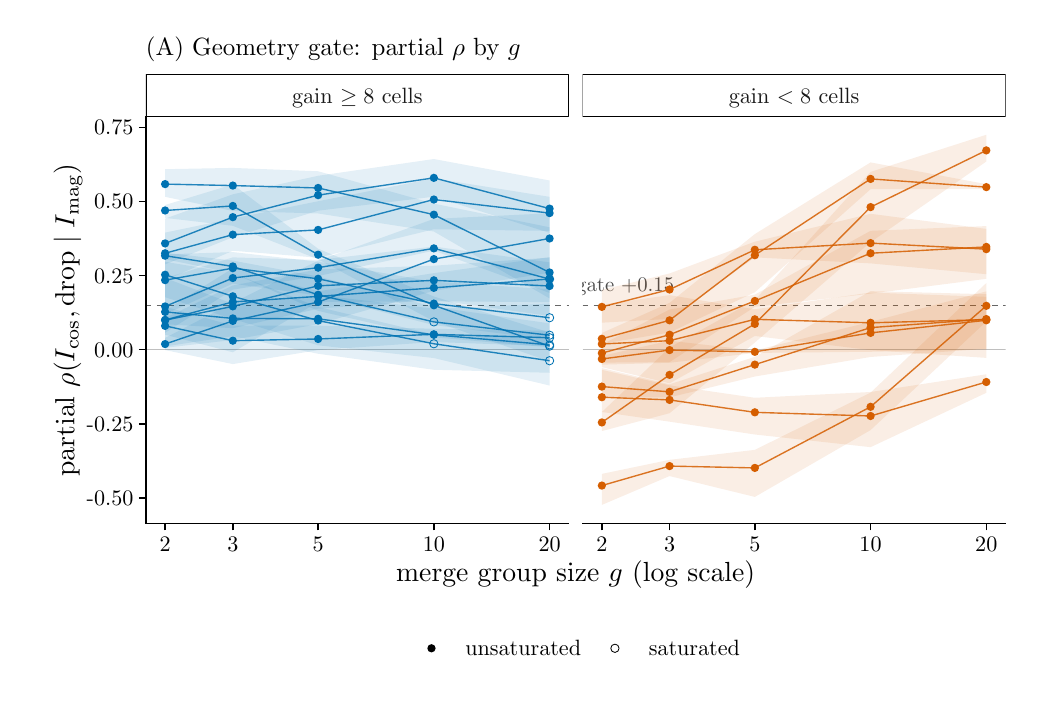
\begin{tikzpicture}[x=1pt,y=1pt]
\definecolor{fillColor}{RGB}{255,255,255}
\path[use as bounding box,fill=fillColor,fill opacity=0.00] (0,0) rectangle (361.35,238.49);
\begin{scope}
\path[clip] (  0.00,  0.00) rectangle (361.35,238.49);
\definecolor{drawColor}{RGB}{255,255,255}
\definecolor{fillColor}{RGB}{255,255,255}

\path[draw=drawColor,line width= 0.5pt,line join=round,line cap=round,fill=fillColor] (  0.00,  0.00) rectangle (361.35,238.49);
\end{scope}
\begin{scope}
\path[clip] ( 42.72, 59.35) rectangle (195.53,206.48);
\definecolor{fillColor}{RGB}{255,255,255}

\path[fill=fillColor] ( 42.72, 59.35) rectangle (195.53,206.48);
\definecolor{drawColor}{gray}{0.40}

\path[draw=drawColor,line width= 0.4pt,dash pattern=on 2pt off 2pt ,line join=round] ( 42.72,138.21) -- (195.53,138.21);
\definecolor{drawColor}{gray}{0.75}

\path[draw=drawColor,line width= 0.3pt,line join=round] ( 42.72,122.14) -- (195.53,122.14);
\definecolor{fillColor}{RGB}{0,114,178}

\path[fill=fillColor,fill opacity=0.10] ( 49.66,137.64) --
	( 74.13,130.84) --
	(104.95,130.81) --
	(146.77,129.69) --
	(188.59,128.94) --
	(188.59,123.41) --
	(146.77,124.91) --
	(104.95,121.98) --
	( 74.13,116.93) --
	( 49.66,121.99) --
	cycle;

\path[] ( 49.66,137.64) --
	( 74.13,130.84) --
	(104.95,130.81) --
	(146.77,129.69) --
	(188.59,128.94);

\path[] (188.59,123.41) --
	(146.77,124.91) --
	(104.95,121.98) --
	( 74.13,116.93) --
	( 49.66,121.99);

\path[fill=fillColor,fill opacity=0.10] ( 49.66,148.04) --
	( 74.13,138.70) --
	(104.95,141.87) --
	(146.77,136.93) --
	(188.59,138.76) --
	(188.59,113.79) --
	(146.77,114.87) --
	(104.95,120.66) --
	( 74.13,127.01) --
	( 49.66,123.31) --
	cycle;

\path[] ( 49.66,148.04) --
	( 74.13,138.70) --
	(104.95,141.87) --
	(146.77,136.93) --
	(188.59,138.76);

\path[] (188.59,113.79) --
	(146.77,114.87) --
	(104.95,120.66) --
	( 74.13,127.01) --
	( 49.66,123.31);

\path[fill=fillColor,fill opacity=0.10] ( 49.66,153.89) --
	( 74.13,149.83) --
	(104.95,137.56) --
	(146.77,127.58) --
	(188.59,126.53) --
	(188.59,109.18) --
	(146.77,119.11) --
	(104.95,123.71) --
	( 74.13,133.26) --
	( 49.66,141.10) --
	cycle;

\path[] ( 49.66,153.89) --
	( 74.13,149.83) --
	(104.95,137.56) --
	(146.77,127.58) --
	(188.59,126.53);

\path[] (188.59,109.18) --
	(146.77,119.11) --
	(104.95,123.71) --
	( 74.13,133.26) --
	( 49.66,141.10);

\path[fill=fillColor,fill opacity=0.10] ( 49.66,169.48) --
	( 74.13,178.27) --
	(104.95,184.96) --
	(146.77,191.02) --
	(188.59,183.27) --
	(188.59,164.36) --
	(146.77,177.41) --
	(104.95,172.36) --
	( 74.13,162.77) --
	( 49.66,152.96) --
	cycle;

\path[] ( 49.66,169.48) --
	( 74.13,178.27) --
	(104.95,184.96) --
	(146.77,191.02) --
	(188.59,183.27);

\path[] (188.59,164.36) --
	(146.77,177.41) --
	(104.95,172.36) --
	( 74.13,162.77) --
	( 49.66,152.96);

\path[fill=fillColor,fill opacity=0.10] ( 49.66,174.40) --
	( 74.13,181.85) --
	(104.95,158.60) --
	(146.77,141.35) --
	(188.59,128.33) --
	(188.59,117.91) --
	(146.77,132.39) --
	(104.95,154.81) --
	( 74.13,166.89) --
	( 49.66,169.76) --
	cycle;

\path[] ( 49.66,174.40) --
	( 74.13,181.85) --
	(104.95,158.60) --
	(146.77,141.35) --
	(188.59,128.33);

\path[] (188.59,117.91) --
	(146.77,132.39) --
	(104.95,154.81) --
	( 74.13,166.89) --
	( 49.66,169.76);

\path[fill=fillColor,fill opacity=0.10] ( 49.66,157.20) --
	( 74.13,154.31) --
	(104.95,148.57) --
	(146.77,137.60) --
	(188.59,131.64) --
	(188.59,122.98) --
	(146.77,126.61) --
	(104.95,136.15) --
	( 74.13,149.81) --
	( 49.66,154.85) --
	cycle;

\path[] ( 49.66,157.20) --
	( 74.13,154.31) --
	(104.95,148.57) --
	(146.77,137.60) --
	(188.59,131.64);

\path[] (188.59,122.98) --
	(146.77,126.61) --
	(104.95,136.15) --
	( 74.13,149.81) --
	( 49.66,154.85);

\path[fill=fillColor,fill opacity=0.10] ( 49.66,156.56) --
	( 74.13,157.40) --
	(104.95,153.91) --
	(146.77,146.67) --
	(188.59,143.98) --
	(188.59,125.82) --
	(146.77,131.03) --
	(104.95,141.69) --
	( 74.13,146.01) --
	( 49.66,134.93) --
	cycle;

\path[] ( 49.66,156.56) --
	( 74.13,157.40) --
	(104.95,153.91) --
	(146.77,146.67) --
	(188.59,143.98);

\path[] (188.59,125.82) --
	(146.77,131.03) --
	(104.95,141.69) --
	( 74.13,146.01) --
	( 49.66,134.93);

\path[fill=fillColor,fill opacity=0.10] ( 49.66,187.35) --
	( 74.13,187.81) --
	(104.95,186.60) --
	(146.77,174.91) --
	(188.59,166.35) --
	(188.59,140.66) --
	(146.77,164.83) --
	(104.95,171.35) --
	( 74.13,172.27) --
	( 49.66,177.36) --
	cycle;

\path[] ( 49.66,187.35) --
	( 74.13,187.81) --
	(104.95,186.60) --
	(146.77,174.91) --
	(188.59,166.35);

\path[] (188.59,140.66) --
	(146.77,164.83) --
	(104.95,171.35) --
	( 74.13,172.27) --
	( 49.66,177.36);

\path[fill=fillColor,fill opacity=0.10] ( 49.66,164.44) --
	( 74.13,169.49) --
	(104.95,175.77) --
	(146.77,184.03) --
	(188.59,177.36) --
	(188.59,165.06) --
	(146.77,165.65) --
	(104.95,155.36) --
	( 74.13,157.89) --
	( 49.66,147.19) --
	cycle;

\path[] ( 49.66,164.44) --
	( 74.13,169.49) --
	(104.95,175.77) --
	(146.77,184.03) --
	(188.59,177.36);

\path[] (188.59,165.06) --
	(146.77,165.65) --
	(104.95,155.36) --
	( 74.13,157.89) --
	( 49.66,147.19);

\path[fill=fillColor,fill opacity=0.10] ( 49.66,126.37) --
	( 74.13,139.08) --
	(104.95,154.31) --
	(146.77,169.39) --
	(188.59,171.42) --
	(188.59,149.92) --
	(146.77,143.42) --
	(104.95,131.38) --
	( 74.13,125.64) --
	( 49.66,122.81) --
	cycle;

\path[] ( 49.66,126.37) --
	( 74.13,139.08) --
	(104.95,154.31) --
	(146.77,169.39) --
	(188.59,171.42);

\path[] (188.59,149.92) --
	(146.77,143.42) --
	(104.95,131.38) --
	( 74.13,125.64) --
	( 49.66,122.81);

\path[fill=fillColor,fill opacity=0.10] ( 49.66,133.56) --
	( 74.13,145.33) --
	(104.95,151.16) --
	(146.77,152.46) --
	(188.59,155.40) --
	(188.59,134.31) --
	(146.77,140.18) --
	(104.95,136.95) --
	( 74.13,129.89) --
	( 49.66,131.33) --
	cycle;

\path[] ( 49.66,133.56) --
	( 74.13,145.33) --
	(104.95,151.16) --
	(146.77,152.46) --
	(188.59,155.40);

\path[] (188.59,134.31) --
	(146.77,140.18) --
	(104.95,136.95) --
	( 74.13,129.89) --
	( 49.66,131.33);

\path[fill=fillColor,fill opacity=0.10] ( 49.66,147.94) --
	( 74.13,155.48) --
	(104.95,154.56) --
	(146.77,159.40) --
	(188.59,153.68) --
	(188.59,142.64) --
	(146.77,157.93) --
	(104.95,148.74) --
	( 74.13,143.83) --
	( 49.66,128.24) --
	cycle;

\path[] ( 49.66,147.94) --
	( 74.13,155.48) --
	(104.95,154.56) --
	(146.77,159.40) --
	(188.59,153.68);

\path[] (188.59,142.64) --
	(146.77,157.93) --
	(104.95,148.74) --
	( 74.13,143.83) --
	( 49.66,128.24);

\path[fill=fillColor,fill opacity=0.10] ( 49.66,136.30) --
	( 74.13,151.53) --
	(104.95,143.20) --
	(146.77,149.79) --
	(188.59,155.57) --
	(188.59,139.30) --
	(146.77,139.63) --
	(104.95,139.34) --
	( 74.13,121.20) --
	( 49.66,127.56) --
	cycle;

\path[] ( 49.66,136.30) --
	( 74.13,151.53) --
	(104.95,143.20) --
	(146.77,149.79) --
	(188.59,155.57);

\path[] (188.59,139.30) --
	(146.77,139.63) --
	(104.95,139.34) --
	( 74.13,121.20) --
	( 49.66,127.56);
\definecolor{drawColor}{RGB}{0,114,178}

\path[draw=drawColor,draw opacity=0.85,line width= 0.5pt,line join=round] ( 49.66,130.73) --
	( 74.13,125.38) --
	(104.95,126.00) --
	(146.77,127.68) --
	(188.59,126.46);

\path[draw=drawColor,draw opacity=0.85,line width= 0.5pt,line join=round] ( 49.66,135.79) --
	( 74.13,133.43) --
	(104.95,133.29) --
	(146.77,127.52) --
	(188.59,123.88);

\path[draw=drawColor,draw opacity=0.85,line width= 0.5pt,line join=round] ( 49.66,149.21) --
	( 74.13,141.42) --
	(104.95,132.64) --
	(146.77,124.27) --
	(188.59,118.14);

\path[draw=drawColor,draw opacity=0.85,line width= 0.5pt,line join=round] ( 49.66,160.53) --
	( 74.13,170.02) --
	(104.95,177.97) --
	(146.77,184.22) --
	(188.59,173.10);

\path[draw=drawColor,draw opacity=0.85,line width= 0.5pt,line join=round] ( 49.66,172.43) --
	( 74.13,174.07) --
	(104.95,156.46) --
	(146.77,138.16) --
	(188.59,123.41);

\path[draw=drawColor,draw opacity=0.85,line width= 0.5pt,line join=round] ( 49.66,156.09) --
	( 74.13,152.21) --
	(104.95,141.97) --
	(146.77,132.17) --
	(188.59,127.36);

\path[draw=drawColor,draw opacity=0.85,line width= 0.5pt,line join=round] ( 49.66,147.26) --
	( 74.13,151.58) --
	(104.95,147.75) --
	(146.77,138.78) --
	(188.59,133.67);

\path[draw=drawColor,draw opacity=0.85,line width= 0.5pt,line join=round] ( 49.66,181.96) --
	( 74.13,181.43) --
	(104.95,180.57) --
	(146.77,170.92) --
	(188.59,150.02);

\path[draw=drawColor,draw opacity=0.85,line width= 0.5pt,line join=round] ( 49.66,156.97) --
	( 74.13,163.70) --
	(104.95,165.41) --
	(146.77,176.39) --
	(188.59,171.49);

\path[draw=drawColor,draw opacity=0.85,line width= 0.5pt,line join=round] ( 49.66,124.16) --
	( 74.13,132.52) --
	(104.95,139.34) --
	(146.77,154.86) --
	(188.59,162.31);

\path[draw=drawColor,draw opacity=0.85,line width= 0.5pt,line join=round] ( 49.66,132.80) --
	( 74.13,137.78) --
	(104.95,145.20) --
	(146.77,147.19) --
	(188.59,145.14);

\path[draw=drawColor,draw opacity=0.85,line width= 0.5pt,line join=round] ( 49.66,137.76) --
	( 74.13,148.02) --
	(104.95,151.77) --
	(146.77,158.74) --
	(188.59,147.65);

\path[draw=drawColor,draw opacity=0.85,line width= 0.5pt,line join=round] ( 49.66,132.88) --
	( 74.13,139.38) --
	(104.95,141.38) --
	(146.77,144.47) --
	(188.59,147.67);
\definecolor{fillColor}{RGB}{0,114,178}

\path[fill=fillColor] ( 49.66,160.53) circle (  1.50);

\path[fill=fillColor] ( 74.13,170.02) circle (  1.50);

\path[fill=fillColor] (104.95,177.97) circle (  1.50);

\path[fill=fillColor] (146.77,184.22) circle (  1.50);

\path[fill=fillColor] (188.59,173.10) circle (  1.50);

\path[fill=fillColor] ( 49.66,172.43) circle (  1.50);

\path[fill=fillColor] ( 74.13,174.07) circle (  1.50);

\path[fill=fillColor] (104.95,156.46) circle (  1.50);

\path[fill=fillColor] (146.77,138.16) circle (  1.50);
\definecolor{drawColor}{RGB}{0,114,178}

\path[draw=drawColor,line width= 0.3pt,line join=round,line cap=round] (188.59,123.41) circle (  1.50);

\path[fill=fillColor] ( 49.66,156.09) circle (  1.50);

\path[fill=fillColor] ( 74.13,152.21) circle (  1.50);

\path[fill=fillColor] (104.95,141.97) circle (  1.50);

\path[draw=drawColor,line width= 0.3pt,line join=round,line cap=round] (146.77,132.17) circle (  1.50);

\path[draw=drawColor,line width= 0.3pt,line join=round,line cap=round] (188.59,127.36) circle (  1.50);

\path[fill=fillColor] ( 49.66,147.26) circle (  1.50);

\path[fill=fillColor] ( 74.13,151.58) circle (  1.50);

\path[fill=fillColor] (104.95,147.75) circle (  1.50);

\path[fill=fillColor] (146.77,138.78) circle (  1.50);

\path[draw=drawColor,line width= 0.3pt,line join=round,line cap=round] (188.59,133.67) circle (  1.50);

\path[fill=fillColor] ( 49.66,181.96) circle (  1.50);

\path[fill=fillColor] ( 74.13,181.43) circle (  1.50);

\path[fill=fillColor] (104.95,180.57) circle (  1.50);

\path[fill=fillColor] (146.77,170.92) circle (  1.50);

\path[fill=fillColor] (188.59,150.02) circle (  1.50);

\path[fill=fillColor] ( 49.66,156.97) circle (  1.50);

\path[fill=fillColor] ( 74.13,163.70) circle (  1.50);

\path[fill=fillColor] (104.95,165.41) circle (  1.50);

\path[fill=fillColor] (146.77,176.39) circle (  1.50);

\path[fill=fillColor] (188.59,171.49) circle (  1.50);

\path[fill=fillColor] ( 49.66,124.16) circle (  1.50);

\path[fill=fillColor] ( 74.13,132.52) circle (  1.50);

\path[fill=fillColor] (104.95,139.34) circle (  1.50);

\path[fill=fillColor] (146.77,154.86) circle (  1.50);

\path[fill=fillColor] (188.59,162.31) circle (  1.50);

\path[fill=fillColor] ( 49.66,132.80) circle (  1.50);

\path[fill=fillColor] ( 74.13,137.78) circle (  1.50);

\path[fill=fillColor] (104.95,145.20) circle (  1.50);

\path[fill=fillColor] (146.77,147.19) circle (  1.50);

\path[fill=fillColor] (188.59,145.14) circle (  1.50);

\path[fill=fillColor] ( 49.66,137.76) circle (  1.50);

\path[fill=fillColor] ( 74.13,148.02) circle (  1.50);

\path[fill=fillColor] (104.95,151.77) circle (  1.50);

\path[fill=fillColor] (146.77,158.74) circle (  1.50);

\path[draw=drawColor,line width= 0.3pt,line join=round,line cap=round] (188.59,147.65) circle (  1.50);

\path[fill=fillColor] ( 49.66,132.88) circle (  1.50);

\path[fill=fillColor] ( 74.13,139.38) circle (  1.50);

\path[fill=fillColor] (104.95,141.38) circle (  1.50);

\path[fill=fillColor] (146.77,144.47) circle (  1.50);

\path[fill=fillColor] (188.59,147.67) circle (  1.50);

\path[fill=fillColor] ( 49.66,130.73) circle (  1.50);

\path[fill=fillColor] ( 74.13,125.38) circle (  1.50);

\path[fill=fillColor] (104.95,126.00) circle (  1.50);

\path[fill=fillColor] (146.77,127.68) circle (  1.50);

\path[draw=drawColor,line width= 0.3pt,line join=round,line cap=round] (188.59,126.46) circle (  1.50);

\path[fill=fillColor] ( 49.66,135.79) circle (  1.50);

\path[fill=fillColor] ( 74.13,133.43) circle (  1.50);

\path[fill=fillColor] (104.95,133.29) circle (  1.50);

\path[fill=fillColor] (146.77,127.52) circle (  1.50);

\path[draw=drawColor,line width= 0.3pt,line join=round,line cap=round] (188.59,123.88) circle (  1.50);

\path[fill=fillColor] ( 49.66,149.21) circle (  1.50);

\path[fill=fillColor] ( 74.13,141.42) circle (  1.50);

\path[fill=fillColor] (104.95,132.64) circle (  1.50);

\path[draw=drawColor,line width= 0.3pt,line join=round,line cap=round] (146.77,124.27) circle (  1.50);

\path[draw=drawColor,line width= 0.3pt,line join=round,line cap=round] (188.59,118.14) circle (  1.50);
\end{scope}
\begin{scope}
\path[clip] (200.53, 59.35) rectangle (353.35,206.48);
\definecolor{fillColor}{RGB}{255,255,255}

\path[fill=fillColor] (200.53, 59.35) rectangle (353.35,206.48);
\definecolor{drawColor}{gray}{0.40}

\path[draw=drawColor,line width= 0.4pt,dash pattern=on 2pt off 2pt ,line join=round] (200.53,138.21) -- (353.35,138.21);
\definecolor{drawColor}{gray}{0.75}

\path[draw=drawColor,line width= 0.3pt,line join=round] (200.53,122.14) -- (353.35,122.14);
\definecolor{drawColor}{gray}{0.30}

\node[text=drawColor,anchor=base,inner sep=0pt, outer sep=0pt, scale=  0.75] at (215.91,143.12) {gate $+0.15$};
\definecolor{fillColor}{RGB}{213,94,0}

\path[fill=fillColor,fill opacity=0.10] (207.48,138.43) --
	(231.94,141.84) --
	(262.76,136.72) --
	(304.58,142.78) --
	(346.40,141.22) --
	(346.40,119.17) --
	(304.58,121.98) --
	(262.76,127.08) --
	(231.94,109.97) --
	(207.48,115.83) --
	cycle;

\path[] (207.48,138.43) --
	(231.94,141.84) --
	(262.76,136.72) --
	(304.58,142.78) --
	(346.40,141.22);

\path[] (346.40,119.17) --
	(304.58,121.98) --
	(262.76,127.08) --
	(231.94,109.97) --
	(207.48,115.83);

\path[fill=fillColor,fill opacity=0.10] (207.48,115.47) --
	(231.94,109.62) --
	(262.76,119.53) --
	(304.58,143.28) --
	(346.40,142.18) --
	(346.40,122.45) --
	(304.58,119.50) --
	(262.76,112.43) --
	(231.94,104.89) --
	(207.48,104.94) --
	cycle;

\path[] (207.48,115.47) --
	(231.94,109.62) --
	(262.76,119.53) --
	(304.58,143.28) --
	(346.40,142.18);

\path[] (346.40,122.45) --
	(304.58,119.50) --
	(262.76,112.43) --
	(231.94,104.89) --
	(207.48,104.94);

\path[fill=fillColor,fill opacity=0.10] (207.48,114.84) --
	(231.94,109.24) --
	(262.76,104.75) --
	(304.58,106.84) --
	(346.40,113.24) --
	(346.40,106.55) --
	(304.58, 86.91) --
	(262.76, 91.48) --
	(231.94, 96.12) --
	(207.48, 99.62) --
	cycle;

\path[] (207.48,114.84) --
	(231.94,109.24) --
	(262.76,104.75) --
	(304.58,106.84) --
	(346.40,113.24);

\path[] (346.40,106.55) --
	(304.58, 86.91) --
	(262.76, 91.48) --
	(231.94, 96.12) --
	(207.48, 99.62);

\path[fill=fillColor,fill opacity=0.10] (207.48, 99.59) --
	(231.94,122.88) --
	(262.76,140.05) --
	(304.58,186.37) --
	(346.40,199.79) --
	(346.40,190.13) --
	(304.58,160.97) --
	(262.76,124.72) --
	(231.94, 99.18) --
	(207.48, 92.72) --
	cycle;

\path[] (207.48, 99.59) --
	(231.94,122.88) --
	(262.76,140.05) --
	(304.58,186.37) --
	(346.40,199.79);

\path[] (346.40,190.13) --
	(304.58,160.97) --
	(262.76,124.72) --
	(231.94, 99.18) --
	(207.48, 92.72);

\path[fill=fillColor,fill opacity=0.10] (207.48,123.98) --
	(231.94,136.63) --
	(262.76,142.02) --
	(304.58,165.08) --
	(346.40,166.79) --
	(346.40,147.73) --
	(304.58,142.39) --
	(262.76,137.62) --
	(231.94,117.65) --
	(207.48,117.46) --
	cycle;

\path[] (207.48,123.98) --
	(231.94,136.63) --
	(262.76,142.02) --
	(304.58,165.08) --
	(346.40,166.79);

\path[] (346.40,147.73) --
	(304.58,142.39) --
	(262.76,137.62) --
	(231.94,117.65) --
	(207.48,117.46);

\path[fill=fillColor,fill opacity=0.10] (207.48,119.90) --
	(231.94,125.37) --
	(262.76,121.84) --
	(304.58,132.19) --
	(346.40,143.20) --
	(346.40,122.28) --
	(304.58,121.37) --
	(262.76,120.96) --
	(231.94,117.41) --
	(207.48,116.71) --
	cycle;

\path[] (207.48,119.90) --
	(231.94,125.37) --
	(262.76,121.84) --
	(304.58,132.19) --
	(346.40,143.20);

\path[] (346.40,122.28) --
	(304.58,121.37) --
	(262.76,120.96) --
	(231.94,117.41) --
	(207.48,116.71);

\path[fill=fillColor,fill opacity=0.10] (207.48, 77.25) --
	(231.94, 82.32) --
	(262.76, 85.93) --
	(304.58,106.61) --
	(346.40,146.22) --
	(346.40,132.32) --
	(304.58, 93.08) --
	(262.76, 68.93) --
	(231.94, 76.47) --
	(207.48, 66.04) --
	cycle;

\path[] (207.48, 77.25) --
	(231.94, 82.32) --
	(262.76, 85.93) --
	(304.58,106.61) --
	(346.40,146.22);

\path[] (346.40,132.32) --
	(304.58, 93.08) --
	(262.76, 68.93) --
	(231.94, 76.47) --
	(207.48, 66.04);

\path[fill=fillColor,fill opacity=0.10] (207.48,128.16) --
	(231.94,139.04) --
	(262.76,163.90) --
	(304.58,189.80) --
	(346.40,181.94) --
	(346.40,180.19) --
	(304.58,180.12) --
	(262.76,142.89) --
	(231.94,128.34) --
	(207.48,124.24) --
	cycle;

\path[] (207.48,128.16) --
	(231.94,139.04) --
	(262.76,163.90) --
	(304.58,189.80) --
	(346.40,181.94);

\path[] (346.40,180.19) --
	(304.58,180.12) --
	(262.76,142.89) --
	(231.94,128.34) --
	(207.48,124.24);

\path[fill=fillColor,fill opacity=0.10] (207.48,143.76) --
	(231.94,149.67) --
	(262.76,161.15) --
	(304.58,171.23) --
	(346.40,165.77) --
	(346.40,149.41) --
	(304.58,153.32) --
	(262.76,155.49) --
	(231.94,133.26) --
	(207.48,131.89) --
	cycle;

\path[] (207.48,143.76) --
	(231.94,149.67) --
	(262.76,161.15) --
	(304.58,171.23) --
	(346.40,165.77);

\path[] (346.40,149.41) --
	(304.58,153.32) --
	(262.76,155.49) --
	(231.94,133.26) --
	(207.48,131.89);
\definecolor{drawColor}{RGB}{213,94,0}

\path[draw=drawColor,draw opacity=0.85,line width= 0.5pt,line join=round] (207.48,124.19) --
	(231.94,125.38) --
	(262.76,133.10) --
	(304.58,131.84) --
	(346.40,132.99);

\path[draw=drawColor,draw opacity=0.85,line width= 0.5pt,line join=round] (207.48,108.79) --
	(231.94,106.90) --
	(262.76,116.73) --
	(304.58,130.10) --
	(346.40,133.18);

\path[draw=drawColor,draw opacity=0.85,line width= 0.5pt,line join=round] (207.48,104.96) --
	(231.94,103.98) --
	(262.76, 99.49) --
	(304.58, 98.17) --
	(346.40,110.45);

\path[draw=drawColor,draw opacity=0.85,line width= 0.5pt,line join=round] (207.48, 95.84) --
	(231.94,113.03) --
	(262.76,131.45) --
	(304.58,173.65) --
	(346.40,194.14);

\path[draw=drawColor,draw opacity=0.85,line width= 0.5pt,line join=round] (207.48,120.89) --
	(231.94,127.54) --
	(262.76,139.74) --
	(304.58,156.98) --
	(346.40,159.27);

\path[draw=drawColor,draw opacity=0.85,line width= 0.5pt,line join=round] (207.48,118.77) --
	(231.94,121.99) --
	(262.76,121.35) --
	(304.58,128.20) --
	(346.40,132.75);

\path[draw=drawColor,draw opacity=0.85,line width= 0.5pt,line join=round] (207.48, 73.03) --
	(231.94, 80.07) --
	(262.76, 79.41) --
	(304.58,101.49) --
	(346.40,137.98);

\path[draw=drawColor,draw opacity=0.85,line width= 0.5pt,line join=round] (207.48,126.07) --
	(231.94,132.74) --
	(262.76,156.27) --
	(304.58,183.84) --
	(346.40,180.87);

\path[draw=drawColor,draw opacity=0.85,line width= 0.5pt,line join=round] (207.48,137.60) --
	(231.94,143.87) --
	(262.76,158.23) --
	(304.58,160.64) --
	(346.40,158.45);
\definecolor{fillColor}{RGB}{213,94,0}

\path[fill=fillColor] (207.48, 95.84) circle (  1.50);

\path[fill=fillColor] (231.94,113.03) circle (  1.50);

\path[fill=fillColor] (262.76,131.45) circle (  1.50);

\path[fill=fillColor] (304.58,173.65) circle (  1.50);

\path[fill=fillColor] (346.40,194.14) circle (  1.50);

\path[fill=fillColor] (207.48,120.89) circle (  1.50);

\path[fill=fillColor] (231.94,127.54) circle (  1.50);

\path[fill=fillColor] (262.76,139.74) circle (  1.50);

\path[fill=fillColor] (304.58,156.98) circle (  1.50);

\path[fill=fillColor] (346.40,159.27) circle (  1.50);

\path[fill=fillColor] (207.48,118.77) circle (  1.50);

\path[fill=fillColor] (231.94,121.99) circle (  1.50);

\path[fill=fillColor] (262.76,121.35) circle (  1.50);

\path[fill=fillColor] (304.58,128.20) circle (  1.50);

\path[fill=fillColor] (346.40,132.75) circle (  1.50);

\path[fill=fillColor] (207.48, 73.03) circle (  1.50);

\path[fill=fillColor] (231.94, 80.07) circle (  1.50);

\path[fill=fillColor] (262.76, 79.41) circle (  1.50);

\path[fill=fillColor] (304.58,101.49) circle (  1.50);

\path[fill=fillColor] (346.40,137.98) circle (  1.50);

\path[fill=fillColor] (207.48,126.07) circle (  1.50);

\path[fill=fillColor] (231.94,132.74) circle (  1.50);

\path[fill=fillColor] (262.76,156.27) circle (  1.50);

\path[fill=fillColor] (304.58,183.84) circle (  1.50);

\path[fill=fillColor] (346.40,180.87) circle (  1.50);

\path[fill=fillColor] (207.48,137.60) circle (  1.50);

\path[fill=fillColor] (231.94,143.87) circle (  1.50);

\path[fill=fillColor] (262.76,158.23) circle (  1.50);

\path[fill=fillColor] (304.58,160.64) circle (  1.50);

\path[fill=fillColor] (346.40,158.45) circle (  1.50);

\path[fill=fillColor] (207.48,124.19) circle (  1.50);

\path[fill=fillColor] (231.94,125.38) circle (  1.50);

\path[fill=fillColor] (262.76,133.10) circle (  1.50);

\path[fill=fillColor] (304.58,131.84) circle (  1.50);

\path[fill=fillColor] (346.40,132.99) circle (  1.50);

\path[fill=fillColor] (207.48,108.79) circle (  1.50);

\path[fill=fillColor] (231.94,106.90) circle (  1.50);

\path[fill=fillColor] (262.76,116.73) circle (  1.50);

\path[fill=fillColor] (304.58,130.10) circle (  1.50);

\path[fill=fillColor] (346.40,133.18) circle (  1.50);

\path[fill=fillColor] (207.48,104.96) circle (  1.50);

\path[fill=fillColor] (231.94,103.98) circle (  1.50);

\path[fill=fillColor] (262.76, 99.49) circle (  1.50);

\path[fill=fillColor] (304.58, 98.17) circle (  1.50);

\path[fill=fillColor] (346.40,110.45) circle (  1.50);
\end{scope}
\begin{scope}
\path[clip] ( 42.72,206.48) rectangle (195.53,221.54);
\definecolor{drawColor}{RGB}{0,0,0}
\definecolor{fillColor}{RGB}{255,255,255}

\path[draw=drawColor,line width= 0.5pt,line join=round,line cap=round,fill=fillColor] ( 42.72,206.48) rectangle (195.53,221.54);
\definecolor{drawColor}{gray}{0.10}

\node[text=drawColor,anchor=base,inner sep=0pt, outer sep=0pt, scale=  0.80] at (119.12,211.26) {gain $\geq 8$ cells};
\end{scope}
\begin{scope}
\path[clip] (200.53,206.48) rectangle (353.35,221.54);
\definecolor{drawColor}{RGB}{0,0,0}
\definecolor{fillColor}{RGB}{255,255,255}

\path[draw=drawColor,line width= 0.5pt,line join=round,line cap=round,fill=fillColor] (200.53,206.48) rectangle (353.35,221.54);
\definecolor{drawColor}{gray}{0.10}

\node[text=drawColor,anchor=base,inner sep=0pt, outer sep=0pt, scale=  0.80] at (276.94,211.26) {gain $< 8$ cells};
\end{scope}
\begin{scope}
\path[clip] (  0.00,  0.00) rectangle (361.35,238.49);
\definecolor{drawColor}{RGB}{0,0,0}

\path[draw=drawColor,line width= 0.5pt,line join=round,line cap=rect] ( 42.72, 59.35) --
	(195.53, 59.35);
\end{scope}
\begin{scope}
\path[clip] (  0.00,  0.00) rectangle (361.35,238.49);
\definecolor{drawColor}{RGB}{0,0,0}

\path[draw=drawColor,line width= 0.5pt,line join=round] ( 49.66, 56.85) --
	( 49.66, 59.35);

\path[draw=drawColor,line width= 0.5pt,line join=round] ( 74.13, 56.85) --
	( 74.13, 59.35);

\path[draw=drawColor,line width= 0.5pt,line join=round] (104.95, 56.85) --
	(104.95, 59.35);

\path[draw=drawColor,line width= 0.5pt,line join=round] (146.77, 56.85) --
	(146.77, 59.35);

\path[draw=drawColor,line width= 0.5pt,line join=round] (188.59, 56.85) --
	(188.59, 59.35);
\end{scope}
\begin{scope}
\path[clip] (  0.00,  0.00) rectangle (361.35,238.49);
\definecolor{drawColor}{RGB}{0,0,0}

\node[text=drawColor,anchor=base,inner sep=0pt, outer sep=0pt, scale=  0.80] at ( 49.66, 49.34) {2};

\node[text=drawColor,anchor=base,inner sep=0pt, outer sep=0pt, scale=  0.80] at ( 74.13, 49.34) {3};

\node[text=drawColor,anchor=base,inner sep=0pt, outer sep=0pt, scale=  0.80] at (104.95, 49.34) {5};

\node[text=drawColor,anchor=base,inner sep=0pt, outer sep=0pt, scale=  0.80] at (146.77, 49.34) {10};

\node[text=drawColor,anchor=base,inner sep=0pt, outer sep=0pt, scale=  0.80] at (188.59, 49.34) {20};
\end{scope}
\begin{scope}
\path[clip] (  0.00,  0.00) rectangle (361.35,238.49);
\definecolor{drawColor}{RGB}{0,0,0}

\path[draw=drawColor,line width= 0.5pt,line join=round,line cap=rect] (200.53, 59.35) --
	(353.35, 59.35);
\end{scope}
\begin{scope}
\path[clip] (  0.00,  0.00) rectangle (361.35,238.49);
\definecolor{drawColor}{RGB}{0,0,0}

\path[draw=drawColor,line width= 0.5pt,line join=round] (207.48, 56.85) --
	(207.48, 59.35);

\path[draw=drawColor,line width= 0.5pt,line join=round] (231.94, 56.85) --
	(231.94, 59.35);

\path[draw=drawColor,line width= 0.5pt,line join=round] (262.76, 56.85) --
	(262.76, 59.35);

\path[draw=drawColor,line width= 0.5pt,line join=round] (304.58, 56.85) --
	(304.58, 59.35);

\path[draw=drawColor,line width= 0.5pt,line join=round] (346.40, 56.85) --
	(346.40, 59.35);
\end{scope}
\begin{scope}
\path[clip] (  0.00,  0.00) rectangle (361.35,238.49);
\definecolor{drawColor}{RGB}{0,0,0}

\node[text=drawColor,anchor=base,inner sep=0pt, outer sep=0pt, scale=  0.80] at (207.48, 49.34) {2};

\node[text=drawColor,anchor=base,inner sep=0pt, outer sep=0pt, scale=  0.80] at (231.94, 49.34) {3};

\node[text=drawColor,anchor=base,inner sep=0pt, outer sep=0pt, scale=  0.80] at (262.76, 49.34) {5};

\node[text=drawColor,anchor=base,inner sep=0pt, outer sep=0pt, scale=  0.80] at (304.58, 49.34) {10};

\node[text=drawColor,anchor=base,inner sep=0pt, outer sep=0pt, scale=  0.80] at (346.40, 49.34) {20};
\end{scope}
\begin{scope}
\path[clip] (  0.00,  0.00) rectangle (361.35,238.49);
\definecolor{drawColor}{RGB}{0,0,0}

\path[draw=drawColor,line width= 0.5pt,line join=round,line cap=rect] ( 42.72, 59.35) --
	( 42.72,206.48);
\end{scope}
\begin{scope}
\path[clip] (  0.00,  0.00) rectangle (361.35,238.49);
\definecolor{drawColor}{RGB}{0,0,0}

\node[text=drawColor,anchor=base east,inner sep=0pt, outer sep=0pt, scale=  0.80] at ( 38.22, 65.79) {-0.50};

\node[text=drawColor,anchor=base east,inner sep=0pt, outer sep=0pt, scale=  0.80] at ( 38.22, 92.59) {-0.25};

\node[text=drawColor,anchor=base east,inner sep=0pt, outer sep=0pt, scale=  0.80] at ( 38.22,119.38) {0.00};

\node[text=drawColor,anchor=base east,inner sep=0pt, outer sep=0pt, scale=  0.80] at ( 38.22,146.18) {0.25};

\node[text=drawColor,anchor=base east,inner sep=0pt, outer sep=0pt, scale=  0.80] at ( 38.22,172.97) {0.50};

\node[text=drawColor,anchor=base east,inner sep=0pt, outer sep=0pt, scale=  0.80] at ( 38.22,199.77) {0.75};
\end{scope}
\begin{scope}
\path[clip] (  0.00,  0.00) rectangle (361.35,238.49);
\definecolor{drawColor}{RGB}{0,0,0}

\path[draw=drawColor,line width= 0.5pt,line join=round] ( 40.22, 68.55) --
	( 42.72, 68.55);

\path[draw=drawColor,line width= 0.5pt,line join=round] ( 40.22, 95.34) --
	( 42.72, 95.34);

\path[draw=drawColor,line width= 0.5pt,line join=round] ( 40.22,122.14) --
	( 42.72,122.14);

\path[draw=drawColor,line width= 0.5pt,line join=round] ( 40.22,148.93) --
	( 42.72,148.93);

\path[draw=drawColor,line width= 0.5pt,line join=round] ( 40.22,175.73) --
	( 42.72,175.73);

\path[draw=drawColor,line width= 0.5pt,line join=round] ( 40.22,202.52) --
	( 42.72,202.52);
\end{scope}
\begin{scope}
\path[clip] (  0.00,  0.00) rectangle (361.35,238.49);
\definecolor{drawColor}{RGB}{0,0,0}

\node[text=drawColor,anchor=base,inner sep=0pt, outer sep=0pt, scale=  1.00] at (198.03, 38.40) {merge group size $g$ (log scale)};
\end{scope}
\begin{scope}
\path[clip] (  0.00,  0.00) rectangle (361.35,238.49);
\definecolor{drawColor}{RGB}{0,0,0}

\node[text=drawColor,rotate= 90.00,anchor=base,inner sep=0pt, outer sep=0pt, scale=  1.00] at ( 16.89,132.91) {partial $\rho(I_{\cos}, \mathrm{drop} \mid I_{\mathrm{mag}})$};
\end{scope}
\begin{scope}
\path[clip] (  0.00,  0.00) rectangle (361.35,238.49);
\definecolor{fillColor}{RGB}{255,255,255}

\path[fill=fillColor] (133.69,  2.00) rectangle (262.38, 26.45);
\end{scope}
\begin{scope}
\path[clip] (  0.00,  0.00) rectangle (361.35,238.49);
\definecolor{fillColor}{RGB}{255,255,255}

\path[fill=fillColor] (138.69,  7.00) rectangle (153.14, 21.45);
\definecolor{fillColor}{RGB}{0,0,0}

\path[fill=fillColor] (145.91, 14.23) circle (  1.50);
\end{scope}
\begin{scope}
\path[clip] (  0.00,  0.00) rectangle (361.35,238.49);
\definecolor{fillColor}{RGB}{255,255,255}

\path[fill=fillColor] (204.98,  7.00) rectangle (219.43, 21.45);
\definecolor{drawColor}{RGB}{0,0,0}

\path[draw=drawColor,line width= 0.3pt,line join=round,line cap=round] (212.20, 14.23) circle (  1.50);
\end{scope}
\begin{scope}
\path[clip] (  0.00,  0.00) rectangle (361.35,238.49);
\definecolor{drawColor}{RGB}{0,0,0}

\node[text=drawColor,anchor=base west,inner sep=0pt, outer sep=0pt, scale=  0.80] at (158.14, 11.47) {unsaturated};
\end{scope}
\begin{scope}
\path[clip] (  0.00,  0.00) rectangle (361.35,238.49);
\definecolor{drawColor}{RGB}{0,0,0}

\node[text=drawColor,anchor=base west,inner sep=0pt, outer sep=0pt, scale=  0.80] at (224.43, 11.47) {saturated};
\end{scope}
\begin{scope}
\path[clip] (  0.00,  0.00) rectangle (361.35,238.49);
\definecolor{drawColor}{RGB}{0,0,0}

\node[text=drawColor,anchor=base west,inner sep=0pt, outer sep=0pt, scale=  0.90] at ( 42.72,228.29) {(A) Geometry gate: partial $\rho$ by $g$};
\end{scope}
\end{tikzpicture}
